\section{Literature Review}
\label{sec:literature}

\subsection{Convolutional Neural Network Architectures}
Convolutional Neural Networks (CNNs) have been a fundamental approach in the field of image processing, particularly in the domain of image segmentation. This section reviews three prominent CNN architectures: Fully Convolutional Networks (FCN), UNet++, and DeepLabV3+, highlighting their innovations, strengths, weaknesses, and typical use cases.

\subsubsection{Fully Convolutional Networks (FCN)}
Introduced by \textit{Long et al.} in 2015, the key innovation of FCN is its fully convolutional nature, which allows it to operate on input images of any size \cite{long2015fcn}. This architecture is simple and flexible, attributed to its use of convolutional layers that replace fully connected layers, enabling the network to efficiently learn spatial hierarchies for pixel-wise segmentation.

\noindent \textbf{Strengths:}
\begin{itemize}
  \item Simple and flexible architecture.
  \item Efficient in learning spatial hierarchies.
\end{itemize}

\noindent \textbf{Weaknesses:}
\begin{itemize}
  \item Produces coarse segmentation maps, lacking in fine detail.
\end{itemize}

\noindent \textbf{Best Use Case:}
\begin{itemize}
  \item General segmentation tasks where detailed precision is less critical.
\end{itemize}

\subsubsection{UNet++}
UNet++ is a more advanced variant that introduces nested dense skip connections to improve the fine-grained segmentation capability, particularly beneficial in medical imaging \cite{zhou2019unet++}. The architecture includes several enhancements such as deep supervision and feature fusion, which allow for more precise and detailed segmentation outputs.

\noindent \textbf{Key Features:}
\begin{itemize}
  \item Nested skip connections facilitate feature refinement across different network layers.
  \item Deep supervision at multiple decoder levels enhances the training dynamics.
  \item Feature fusion through decoder nodes integrates information from multiple preceding layers.
\end{itemize}

\noindent \textbf{Advantages:}
\begin{itemize}
  \item Achieves fine-grained segmentation, crucial for medical applications.
  \item Manages computational costs effectively compared to more complex models.
\end{itemize}

\noindent \textbf{Weakness:}
\begin{itemize}
  \item Slightly higher computational overhead than basic UNet due to additional connections.
\end{itemize}

\noindent \textbf{Best Use Case:}
\begin{itemize}
  \item High-resolution medical image segmentation where detail is paramount.
\end{itemize}

\subsubsection{DeepLabV3+}
DeepLabV3+, developed by \textit{Chen et al.}, incorporates atrous convolution and an atrous spatial pyramid pooling (ASPP) module to effectively capture multi-scale contextual information \cite{chen2018deeplabv3+}. This design allows the network to handle complex scenes with varying object scales efficiently.

\noindent \textbf{Strengths:}
\begin{itemize}
  \item Handles multiple scales effectively using ASPP.
  \item Suitable for complex scene segmentation with high variability in object size and structure.
\end{itemize}

\noindent \textbf{Weaknesses:}
\begin{itemize}
  \item Computationally intensive, requiring significant resources.
\end{itemize}

\noindent \textbf{Best Use Case:}
\begin{itemize}
  \item Complex scene segmentation such as urban landscapes or densely populated images.
\end{itemize}

\subsection{UNet++}
UNet++ is an enhanced structure of the traditional UNet model designed to achieve more accurate segmentation, especially in medical imaging applications. It introduces several innovative concepts:

\paragraph{Nested Skip Connections}
These connections are comprised of multiple intermediate nodes that refine and combine features from various network paths, enhancing the network's ability to propagate context and capture detailed structures within the image.

\paragraph{Deep Supervision}
UNet++ incorporates output layers attached at multiple decoder levels, facilitating the direct influence of the loss function across different depths of the network. This approach helps in the faster convergence of the network and improves the gradient flow, leading to enhanced learning capabilities.

\paragraph{Feature Fusion}
The decoder nodes in UNet++ integrate information from both preceding layers and skip connections. This fusion occurs via up-sampling and convolutions, allowing the network to preserve essential details and improve the quality of the segmentation output.

\begin{figure}[h]
\centering
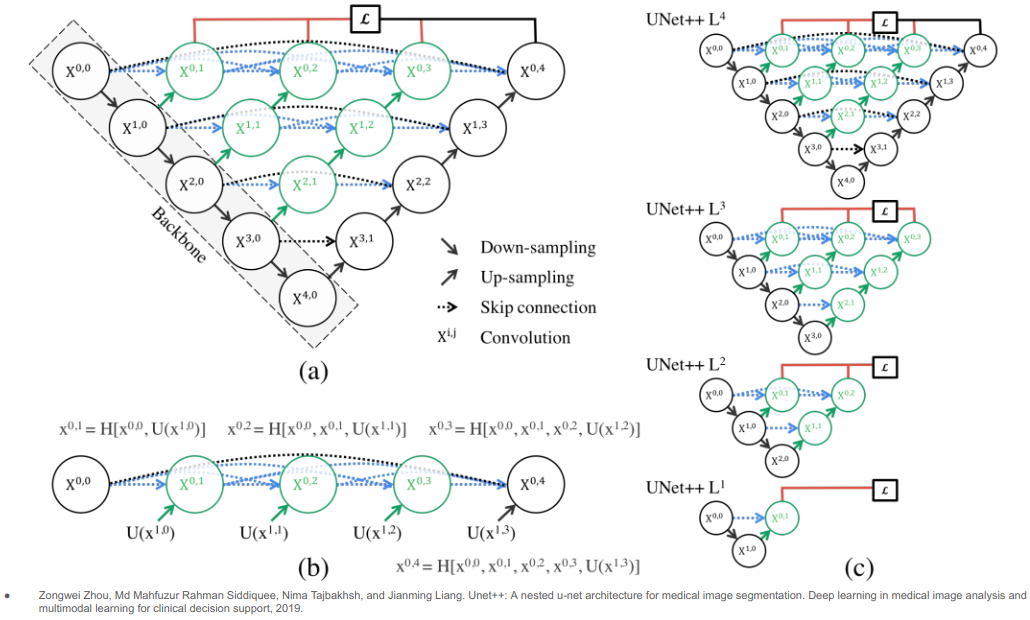
\includegraphics[width=0.48\textwidth]{images/unet_plus_architecture.png}
\caption{The architecture of UNet++ showing nested skip connections, deep supervision, and feature fusion mechanisms.}
\label{fig:unet_plus_architecture}
\end{figure}

\paragraph{Mathematical Formulation}
The operations within the UNet++ can be described by the following equation:
\[
F_{i,j} = H_{i,j} \left( F_{i-1,j} + \sum_{k=0}^{j-1} H_{i,k} \right)
\]
where \( F_{i,j} \) represents the feature map at the \( j^{th} \) node of the \( i^{th} \) layer, \( H_{i,j} \) is the convolution operation at node \( j \) of layer \( i \), and the summation aggregates the feature maps from all previous nodes at the same layer, enhancing the feature integration across the network.

\paragraph{Advantages}
\begin{itemize}
    \item UNet++ is capable of capturing detailed features such as water boundaries, which is critical for applications like flood area segmentation.
    \item It performs well on smaller datasets, a common limitation in specialized fields such as medical imaging, where large annotated datasets may not be available.
    \item The computation cost, while higher than simpler architectures like FCN, remains manageable and less intensive compared to more complex models like DeepLabV3+.
\end{itemize}

\paragraph{Applications}
UNet++ is particularly suited for high-resolution image tasks where detailed feature delineation is critical. It has shown promising results in medical imaging, including tasks like tumor segmentation and organ delineation.

\subsection{Graph Neural Networks: Graph-FCN and CNN-G}

Deep learning has made significant advancements in semantic segmentation by classifying pixels in images. However, during high-level feature extraction, it often ignores the local spatial information, which is important for accurate segmentation. Graph-based models address this limitation by including the missing local context.

\subsubsection{Graph-FCN}

Graph-FCN combines graph convolutional networks (GCNs) with fully convolutional networks (FCNs) to capture local spatial relationships in images. Initially, a convolutional network converts the image grid data into a graph structure, transforming the semantic segmentation task into a graph node classification problem. The graph convolutional network is then applied to classify the nodes in this graph, effectively solving the segmentation challenge.

FCN-16s generates feature maps, and node annotations are initialized by combining upsampled feature vectors and node locations. Labels for nodes are obtained by pooling the raw label image during training. The process is shown in Figure~\ref{fig:graphfcn_node_init}.

\begin{figure}
    \centering
    % \fbox{\rule{0pt}{2in} \rule{0.9\linewidth}{0pt}}
    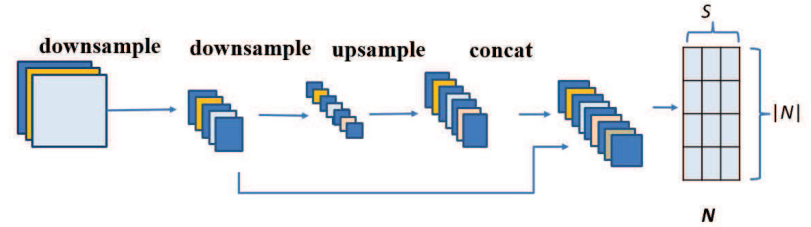
\includegraphics[width=0.8\linewidth]{images/graphfcn_node_init.png}
    \caption{Graph-FCN node initialization. From ~\cite{lu2020graphfcnimagesemanticsegmentation}.}
    \label{fig:graphfcn_node_init}
\end{figure}

In the graph model, edges are represented by an adjacency matrix, where each node is connected to its nearest $l$ nodes. These connections allow node annotations to transfer through the edges in the graph neural network.

FCN-16s handles node classification and graph model initialization on a small feature map, while a 2-layer GCN classifies the nodes within the graph. Cross-entropy loss is computed for both outputs, and like FCN-16s, Graph-FCN is trained end-to-end. The output of the prediction process is the output of the convolutional network. The graph model is only used during the training.

The structure of the Graph-FCN model is shown in Figure~\ref{fig:graphfcn_structure}.
\begin{figure}
    \centering
    % \fbox{\rule{0pt}{2in} \rule{0.9\linewidth}{0pt}}
    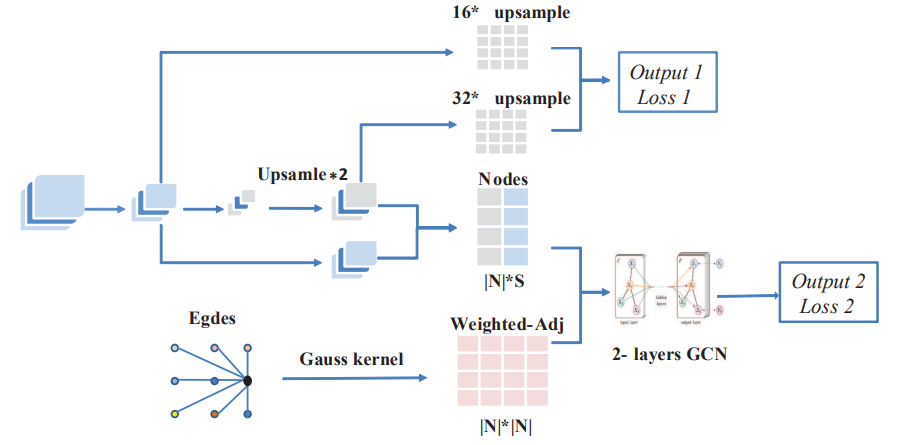
\includegraphics[width=0.8\linewidth]{images/graphfcn_structure.png}
    \caption{Graph-FCN model structure. From ~\cite{lu2020graphfcnimagesemanticsegmentation}.}
    \label{fig:graphfcn_structure}
\end{figure}

\subsubsection{CNN-G}

CNN-G builds on the Graph-FCN model by incorporating a graph-based approach with a convolutional neural network. Two types of structure models are used in CNN-G: distance-based and semantic-based, solved by GCN and GAT, respectively. The distance-based model captures the spatial relationships between nodes, while the semantic-based model focuses on the semantic relationships.

Using a graph attention network (GAT) enables flexible feature extraction across various receptive fields. This approach allows the model to integrate both structure learning and feature extraction.

\textbf{Distance-Based Structure:} Based on the assumption that the closer nodes are more correlated, the Gauss kernel function is used to generate the weighted edges.

The adjacent matrix $A = [e_{ij}]_{|N| \times |N|}$ is used to represent the edge set:

\[
e_{ij} = \begin{cases} \exp \left( -\frac{\|p_i - p_j\|^2}{\sigma^2} \right), & \text{an edge between } n_i \text{ and } n_j \\ 0, & \text{otherwise} \end{cases}.
\]

To simplify the calculation, we make the nodes connect to the $l$ closest nodes.

\textbf{Semantic-based model:} The initial attention coefficient $c_{ij}$ is used to measure the correlation between two nodes. The features of nodes with the same category will be more similar, the attention coefficient between each other will be larger, and the similarity is gradually strengthened in the iteration. A linear transformation is taken to map the concatenation of two nodes' features into a real number: 
\[
c_{ij} = a \left( n_i' || n_j' \right)
\]
The final attention coefficient is obtained through the normalization of all neighborhood nodes: 
\[
e_{ij} = \frac{\exp(c_{ij})}{\sum_{k \in neib_{i}} \exp(c_{ik})}.
\]
When the graph structure is unknown, the matrix $A_{\text{att}} = [e_{ij}]_{|N| \times |N|}$ can be taken as the adjacency matrix. In this case, the edge set is generated by the calculation of the attention coefficients.

In each case, the model generates two outputs, $y1$ and $y2$, which corresponds to two losses, $loss1$ and $loss2$. Both share the convolutional layer's extracted features. The final prediction is based on $y1$. Similar to Graph-FCN, the graph model is only used during training.

The structure of the CNN-G model is shown in Figure~\ref{fig:cnng_structure}.
\begin{figure}
    \centering
    % \fbox{\rule{0pt}{2in} \rule{0.9\linewidth}{0pt}}
    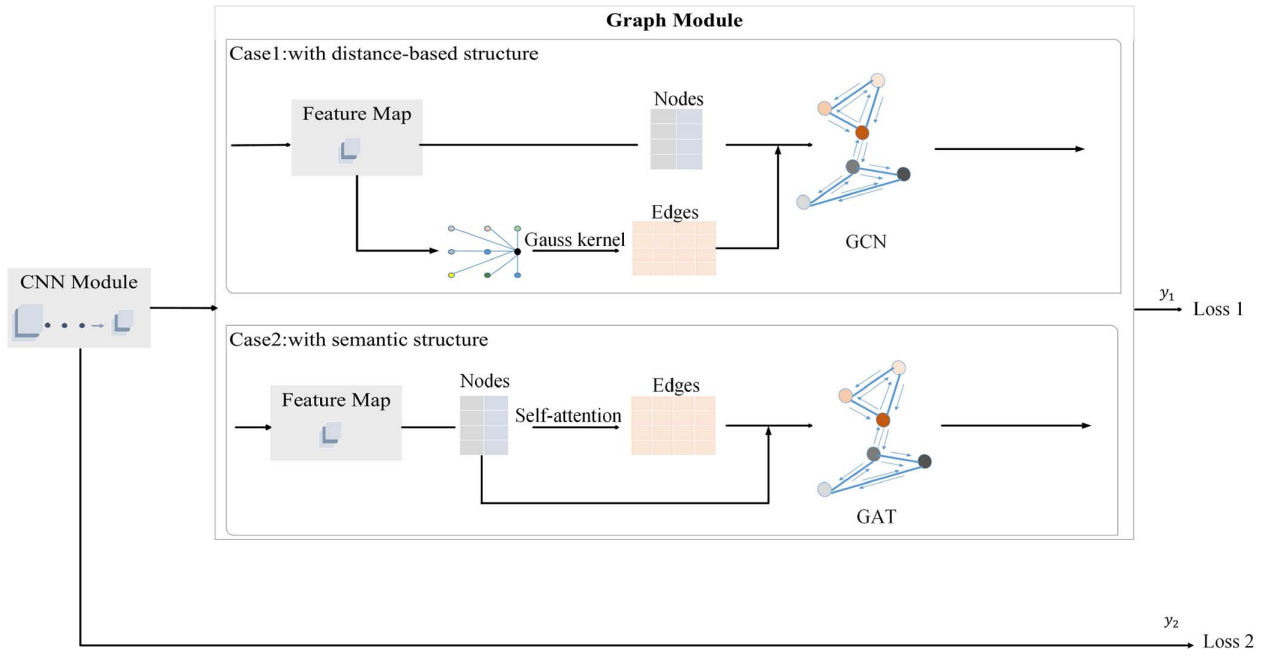
\includegraphics[width=0.8\linewidth]{images/cnng_structure.png}
    \caption{CNN-G model structure. From ~\cite{9103557}.}
    \label{fig:cnng_structure}
\end{figure}

\subsection{Transformer}
\subsubsection{TransUnet}
TransUNet \cite{chen2021transunettransformersmakestrong} has emerged as a robust framework for medical image segmentation by combining the strengths of U-Net and Transformer architectures. Refer the figure \ref{fig:transunet} for the architecture diagram.

\begin{figure}[t]
    \centering
     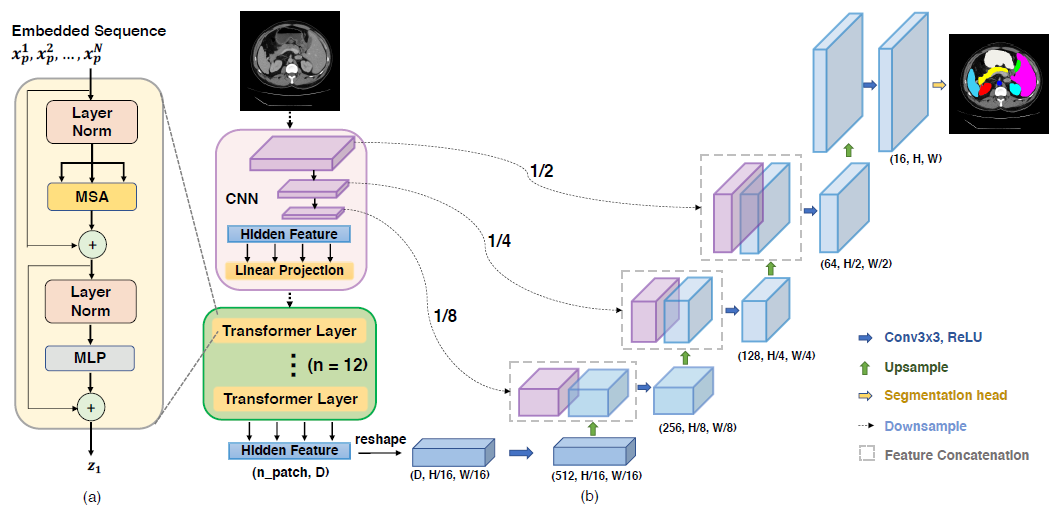
\includegraphics[width=0.9\linewidth]{images/transUnet_arch.png}
  
     \caption{TransUnet architecture. From ~\cite{chen2021transunettransformersmakestrong}.}
     \label{fig:transunet}
\end{figure}

TransUNet addresses these limitations by introducing a hybrid architecture that leverages both CNNs and Transformers. The encoder consists of a CNN followed by a Transformer module. The CNN is used to extract feature maps from the input images, which are then tokenized into image patches and fed into the Transformer. This CNN-Transformer hybrid allows TransUNet to capture detailed spatial features (via CNN) and global context (via the Transformer) simultaneously.

In the decoder, a cascaded upsampling module (CUP) is employed, consisting of multiple upsampling blocks with convolutional layers and ReLU activation. These upsampled features are combined with the high-resolution CNN feature maps from the encoder through skip connections, similar to the U-Net structure, enabling precise localization. This U-Net-like design ensures that TransUNet can recover lost spatial detail while preserving the high-level semantic understanding captured by the Transformer.
\subsubsection{MaskFormer}
Image segmentation models which can solve all 3 tasks (instance, semantic and panoptic segmentation) with a unified architecture started to appear in the literature in the last few years. This started with \underline{DETR} \cite{carion2020endtoendobjectdetectiontransformers} and later improved by \underline{MaskFormer} \cite{cheng2021perpixelclassificationneedsemantic} for semantic segmentation.

\underline{Mask2Former} \cite{cheng2022maskedattentionmasktransformeruniversal}, which adopts the
same meta architecture as MaskFormer, with a backbone, a pixel decoder and a Transformer decoder, extends this to instance segmentation by further improving the neural network architecture in the following ways:
\begin{itemize}
    \item \textbf{Masked Attention}: They use \textit{masked attention} (rather than the standard cross-attention) in the Transformer decoder which restricts the attention to localized features centered around predicted segments, which can be either objects or regions depending on the specific semantic for grouping.
    \item \textbf{Multi-scale high-resolution features}: High-resolution features improve model performance, especially for small objects. However, this is computationally demanding. Therefore, instead of always using the high-resolution feature map, they utilize a feature pyramid which consists of both low and high-resolution features and feed one resolution of the multi-scale feature to one Transformer decoder layer at a time.
\end{itemize}
It also made improvements in optimization and training strategies. The architecture diagram is given in Figure \ref{fig:mask2former}.

\begin{figure}[t]
    \centering
     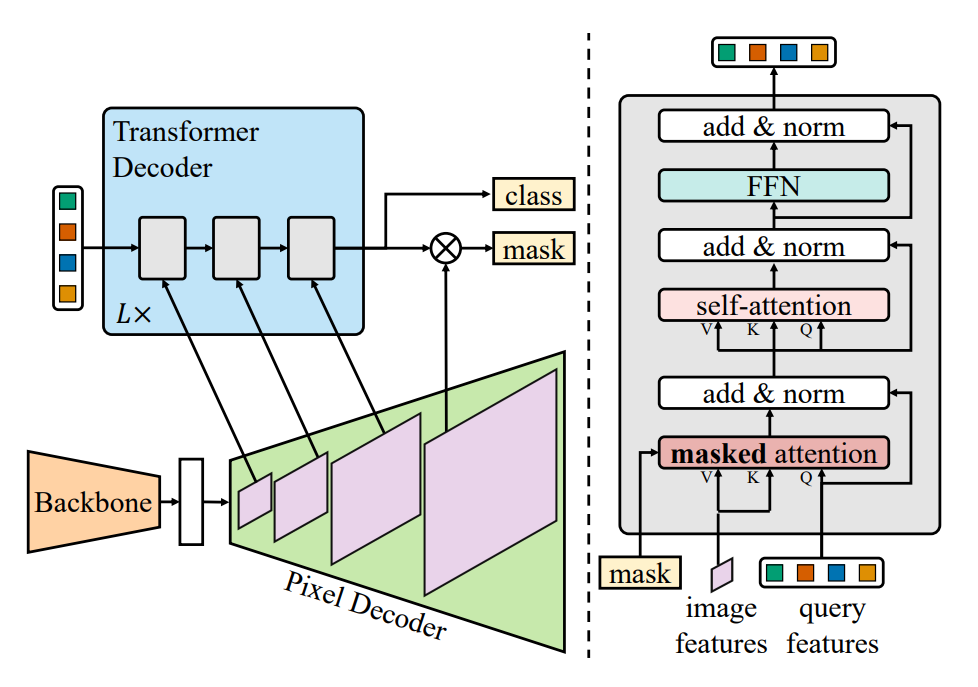
\includegraphics[width=0.8\linewidth]{images/mask2former_arch.png}
  
     \caption{Mask2Former architecture. From ~\cite{cheng2022maskedattentionmasktransformeruniversal}.}
     \label{fig:mask2former}
\end{figure}